\chapter{FLEXIBLE TOOLS FOR AMBER SIMULATIONS}
\label{ch6}

In this chapter, I will describe the motivation behind creating two tools to aid
users in carrying out biomolecular simulations with the Amber programming
package as well as some details regarding their functionality and
implementation. During the course of my graduate studies, I wrote several
scripts and programs to aid in my work---several of which I polished and released
with the Amber suite of programs. The two I will describe in this chapter are
\emph{MMPBSA.py} \cite{MMPBSApy} and \emph{ParmEd}.

\section{MMPBSA.py}

Portions of this section are reprinted with permission from
\citeauthor*{MMPBSApy}, ``MMPBSA.py: An Efficient Program for End-State Free
Energy Calculations,'' \emph{J. Chem. Theory Comput.}, 2012, \textbf{8} (9), pp
3314--3321. \cite{MMPBSApy}

\emph{MMPBSA.py} is a script designed to automate the procedure of performing
end-state free energy calculations, as described in Sec. \ref{sec1:MMPBSA}.

\subsection{Motivation}

End-state free energy methods---briefly described in Sec.
\ref{sec1:EndState}---are popular methods for computing binding free energies
for protein-ligand binding, \cite{Wang2001, Kuhn2005, Weis2006, Genheden2009,
Wang2001a} protein-protein binding, \cite{Gohlke2003, Gohlke2004, Bradshaw2010,
Wang2001a} nucleic acid binding, \cite{Gouda2002, Wang2001a} and relative
conformational stabilities. \cite{Combelles2008, Brice2011} There has been
significant effort applied to improving the approximations used in end-state
methods, and in some cases it has even approached predictive accuracy.
\cite{Genheden2009, Mikulskis2012}

By 2008, there was a set of perl scripts capable of automating MM-PBSA and
MM-GBSA calculations that were written in 2002 for release with Amber 7 and had
not been changed since 2003. These scripts will be collectively referred to as
\emph{mm\_pbsa.pl} from now on. Due to its age, \emph{mm\_pbsa.pl} was
compatible only with the low-precision, inefficient ASCII trajectory format,
and offered only a limited set of the available implicit solvent models and
input parameters that had been developed over the decade that followed its
initial release. Furthermore, the input for \emph{mm\_pbsa.pl} was very
different from the typical input that most other Amber programs expected.
Finally, \emph{mm\_pbsa.pl} was only capable of running in serial, despite the
fact that end-state analyses themselves could be trivially parallelized by
computing binding free energies for individual frames simultaneously.

The goal of my project was to revitalize this set of helpful scripts that had
fallen out of support and had grown outdated. We wanted to bring the input style
in line with the rest of the Amber programs---for example, atom selections
should be input via the Amber mask syntax, and groups of related variables
should be specified in Fortran-style namelists. Furthermore, we wanted to
provide the user with access to new input variables and solvent models. Given
the magnitude of the changes required, the recent emergence of Python in the
field of computational chemistry, \cite{Sanner1999, Cock2009,
Michaud-Agrawal2011, MMPBSApy} and the undocumented, monolithic state of
\emph{mm\_pbsa.pl}, we decided to build a new script to perform end-state free
energy calculations in Python---\emph{MMPBSA.py}. \cite{MMPBSApy}

\subsection{Capabilities}

In this section, I will briefly outline some of the various types of
calculations that \emph{MMPBSA.py} is capable of performing.

\subsubsection{Stability and Binding Free Energy Calculations}

End-state calculations are frequently used for two types of
analyses---calculating the relative stability of multiple conformations of a
system and calculating the binding free energy in a non-covalently bound,
receptor-ligand complex, \cite{Homeyer2012} whose thermodynamic cycles were
shown in Ch. \ref{ch2}, Fig. \ref{fig2:MMPBSA}. Stability calculations compare
the free energies of multiple conformations to determine their relative
stability. If we consider the process of a biomolecule changing conformations
from state A to state B, then the free energy associated with that
conformational change is simply the difference in the free energies of states A
and B. Similarly, the non-covalent binding free energies can be computed as the
difference in free energies of the bound and free states of the two species in
solution.

The free energy changes in solution can be decomposed according to
\begin{equation}
   \Delta G_{solvated} = E_{gas} + \Delta G_{solvation} - T \Delta S_{solute}
   \label{eq6:GSolv}
\end{equation}
where $\Delta G_{solvation}$ represents a true free energy, since the solvent
degrees of freedom have been averaged by using an implicit solvent model. The
free energy of solvation in \ref{eq6:GSolv} can be further decomposed into a sum
of polar and non-polar contributions in most implicit solvent models. Among the
solvent models available for end-state calculations in \emph{MMPBSA.py} are the
previously mentioned PB and GB implicit solvent models as well as the
3-dimensional reference interaction site model (3D-RISM). \cite{Genheden2010}

The energies described in Eq. \ref{eq6:GSolv} are single point energies of the
system. However, in practice, end-state calculations estimate these energies
according to ensemble averages taken from a simulation. Expressing Eq.
\ref{eq6:GSolv} in terms of an average over a simulated ensemble yields Eq.
\ref{eq6:GSolvAvg}.

\begin{align}
   \Delta G_{solvated} & \approx \left \langle E_{gas} \right \rangle + \left
         \langle \Delta G_{solvation} \right \rangle - T \left \langle
         S_{solute} \right \rangle \nonumber \\
   & = \frac 1 N \left \lbrace \sum_{i=1}^N \left[E_{i,gas} + \Delta
         G_{i,solvation} \right] - T\sum_{i=1}^N S_{i,solute} \right \rbrace
   \label{eq6:GSolvAvg}
\end{align}
where $i$ is the index of a particular frame and $N$ is the total number of
analyzed frames.

There are two approaches to generating the necessary ensembles for the bound and
unbound state of binding energy calculations---all ensembles can be extracted
from a single MD or MC trajectory of the bound complex, or trajectories can be
generated for each state using separate simulations. \cite{Wang2006} These
approaches are called the \emph{single trajectory protocol} (STP) and the
\emph{multiple trajectory protocol} (MTP), respectively, and each approach has
distinct advantages and disadvantages.

STP is less computationally expensive than MTP, because only a single trajectory
is required to generate all three ensembles. Furthermore, the internal potential
terms (e.g., bonds, angles, and torsions) cancel exactly in the STP, because
the conformations in the bound and unbound ensembles are the same, leading to
lower fluctuations and easier convergence in the binding free energy. The STP is
appropriate if the receptor and ligand ensembles are comparable in the bound and
unbound states. However, the conformations populating the unbound ensembles
typically adopt strained configurations when extracted from the bound state
ensemble, thereby over-stabilizing the binding, compared to the MTP.

\subsubsection{Free Energy Decomposition}

Amber \cite{AMBER12} provides several schemes to decompose calculated free
energies into specific residue contributions using either the GB or PB implicit
solvent models, \cite{Metz2012} following the work of \citeauthor{Gohlke2003}
\cite{Gohlke2003} Interactions can be decomposed for each residue by including
only those interactions in which one of the residue's atoms is involved---a
scheme called \emph{per-residue} decomposition. Alternatively, interactions can
be decomposed by specific residue pairs by including only those interactions in
which one atom from each of the analyzed residues is participating---a scheme
called \emph{pairwise} decomposition. These decomposition schemes can provide
useful insights into important interactions in free energy calculations.
\cite{Gohlke2003}

However, it is important to note that solvation free energies using GB and PB
are not strictly pairwise decomposable, since the dielectric boundary defined
between the protein and the bulk solvent is inherently nonlocal and depends on
the arrangement of all atoms in space. Thus, care must be taken when
interpreting free energy decomposition results.

An alternative way of decomposing free energies is to introduce specific
mutations in the protein sequence and analyze how binding free energies or
stabilities are affected. \cite{Massova2000} Alanine scanning, which is a
technique in which an amino acid in the system is mutated to alanine, can
highlight the importance of the electrostatic and steric nature of the original
side chain. \cite{Massova1999} Assuming that the mutation will have a negligible
effect on protein conformation, we can incorporate the mutation directly into
each member of the original ensemble. This avoids the need to perform an
additional MD or MC simulation to generate an ensemble for the mutant.

\subsubsection{Entropy Calculations}

The implicit solvent models used to calculate relative stability and binding
free energies in end-state calculations often neglect some contributions to the
solute entropy. If we assume that biological systems obey a rigid rotor model,
we can calculate the translational and rotational entropies using standard
statistical mechanical formulae, \cite{McQuarrie_Book_StatMech_1973} and we can
approximate the vibrational entropy contribution using one of two methods.
First, the vibrational frequencies of normal modes can be calculated at various
local minima of the potential energy surface.
\cite{McQuarrie_Book_StatMech_1973} Alternatively, the eigenvalues of the
mass-weighted covariance matrix constructed from every member of the ensemble
can be approximated as frequencies of global, orthogonal motions---a technique
called the \emph{quasi-harmonic} approximation.
\cite{Brooks_JComputChem_1995_v16_p1522} Using either the normal mode or
quasi-harmonic approximations, we can sum the vibrational entropies of each mode
calculated from standard formulae. \cite{McQuarrie_Book_StatMech_1973}

Typically, normal mode calculations are computationally demanding for large
systems, because they require minimizing every frame, building the Hessian
matrix, and diagonalizing it to obtain the vibrational frequencies
(eigenvalues). Because of the Hessian diagonalization, normal-mode calculations
scale as roughly $(3N)^3$, where N is the number of atoms in the system. While the
quasi-harmonic approach is less computationally expensive, a large number of
snapshots are typically needed to extrapolate the asymptotic limit of the total
entropy for each ensemble, which increases the computational cost of the
original simulation. \cite{Wang2001}

\subsection{General Workflow}

\emph{MMPBSA.py} is a program written in Python and \emph{nab}
\cite{Macke_BookChap_MolModNucAcid_2000_p379} that streamlines the procedure of
preparing and calculating free energies for an ensemble generated by MD or MC
simulations whose general workflow is shown in Fig. \ref{fig6:MMPBSA_Workflow}.
The process of calculating binding free energies can be a tedious procedure that
\emph{MMPBSA.py} aims to shorten and simplify.

Python is a useful programming language for performing tasks that are not
numerically intensive, and because it is available on virtually every platform,
Python programs are highly portable. Nucleic Acid Builder (\emph{nab}),
\cite{Macke_BookChap_MolModNucAcid_2000_p379} which is a molecule-based
programming language included with AmberTools, contains functionality pertinent
to building, manipulating and performing energy calculations on biological
systems, such as proteins and nucleic acids.

\begin{figure}
   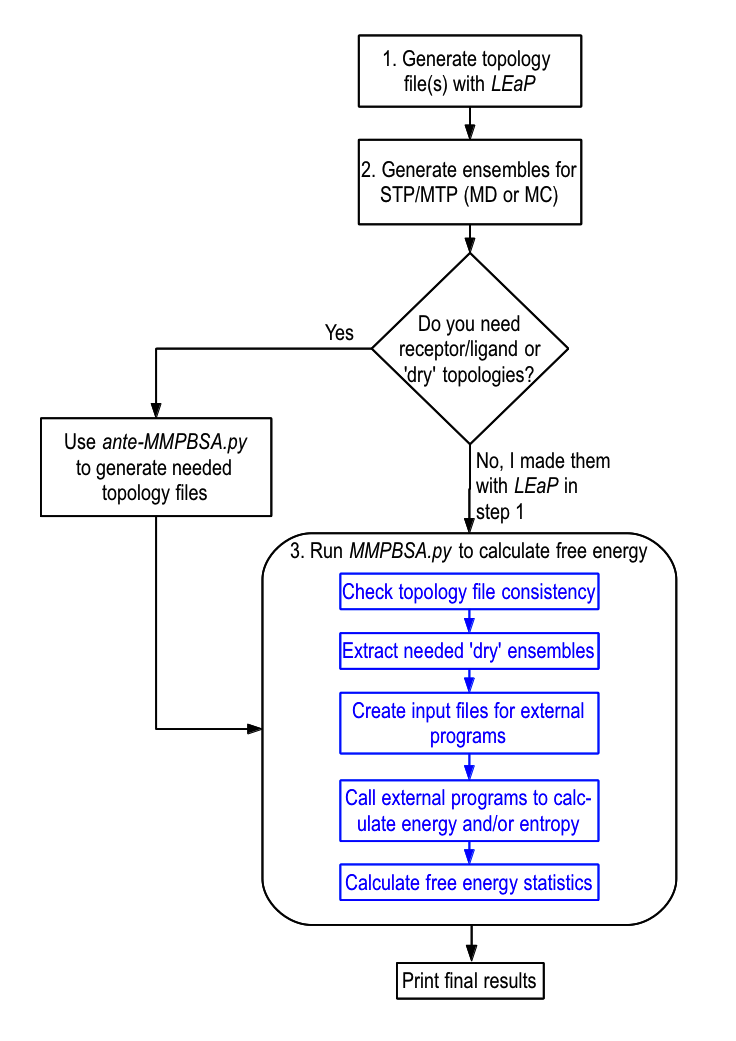
\includegraphics[height=6in, width=4.24in]{MMPBSA_Workflow.png}
   \caption[General workflow for performing end-state calculations with
            \emph{MMPBSA.py}. LEaP is a program in Amber used to create topology
            files for dynamics.]
           {General workflow for performing end-state calculations with
            \emph{MMPBSA.py}. LEaP is a program in Amber used to create topology
            files for dynamics. The workflow shown in step 3 is the series of
            steps that \emph{MMPBSA.py} automates. ``Dry'' topologies and
            ensembles are systems without explicit solvent that are subsequently
            treated using an implicit solvent model. ``External programs''
            refers to the executables that perform the energy calculations (\eg
            \emph{sander}).}
   \label{fig6:MMPBSA_Workflow}
\end{figure}

End-state calculations often require multiple \emph{topology files} (described
later) that contain the parameters corresponding to the force field. Simulations
are typically run using explicit solvent with any of the electrostatics methods
described in Ch. \ref{ch2}, which would require both solvated and unsolvated
topology files to use with \emph{MMPBSA.py}. It is necessary that all topology
files have a consistent set of parameters, especially for binding free energy
calculations. Therefore, \emph{MMPBSA.py} checks the input topology files prior
to binding free energy calculations to prevent erroneous results due to
inconsistencies that may not be immediately obvious (\eg different particle
counts, partial charges for the same atoms, etc.). I wrote the Python utility
\emph{ante-MMPBSA.py} (also released alongside \emph{MMPBSA.py}), which allows a
user to easily create topology files with a consistent set of parameters,
including changing the intrinsic implicit solvent radius set to fit the desired
solvent model.

The use of \emph{MMPBSA.py} is similar to that of Amber's MD engines
\emph{sander} and \emph{pmemd}. The command-line flags common to both
\emph{MMPBSA.py} and the MD engines are identical, and input files are separated
with similar, Fortran-style namelists, indicated with an ampersand (\&) prefix.

The \emph{MMPBSA.py} input file contains a &general namelist for variables that
control general behavior. For example, variables that control the subset of
frames analyzed (startframe, endframe, and interval) and the amount of
information printed in the output file (verbose) are specified here. An example
of this section is shown below:
\begin{verbatim}
General MMPBSA.py input file
&general
   startframe=1, endframe=100, interval=2,
   keep_files=0, verbose=1, strip_mask=:WAT:Cl-:Na+,
/
\end{verbatim}

\subsection{Running in Parallel}

\emph{MMPBSA.py} is implemented in parallel, so users with access to multiple
processors can speed up their calculations. \emph{MMPBSA.py.MPI} is the parallel
implementation of \emph{MMPBSA.py} that uses MPI (described in Appendix
\ref{appendixC}) for Python (\emph{mpi4py}). Since energy calculations for each
frame are independent, the calculation can be trivially parallelized, given
enough available processors. \emph{MMPBSA.py.MPI} divides frames evenly across
all processors, which allows calculations using many frames to scale better than
if \emph{MMPBSA.py} invoked parallel executables to calculate free energies.
However, perfect scaling is not attained, because certain setups tasks and file
input/output can only be done with a single processor. Fig.
\ref{fig6:MMPBSA_Scaling} demonstrates scaling for a sample MM-PBSA and MM-GBSA
calculation.

\begin{figure}
   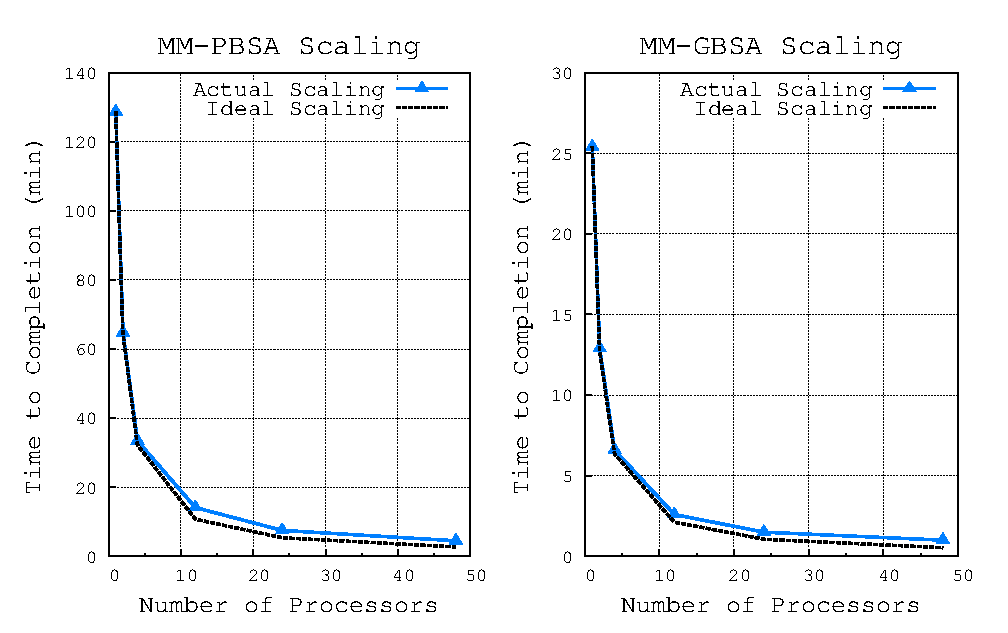
\includegraphics[width=6.5in]{MMPBSA_Scaling.eps}
   \caption[\emph{MMPBSA.py} scaling comparison for MM-PBSA and MM-GBSA
            calculations on 200 frames of a 5910-atom complex.]
           {\emph{MMPBSA.py} scaling comparison for MM-PBSA and MM-GBSA
            calculations on 200 frames of a 5910-atom complex. Times shown are
            the times required for the calculation to finish. Note that MM-GBSA
            calculations are $\sim$5 times faster than MM-PBSA calculations. All
            calculations were performed on NICS Keeneland (2 Intel Westmere
            6-core CPUs per node, QDR infiniband interconnect).}
   \label{fig6:MMPBSA_Scaling}
\end{figure}

\subsection{Differences to \emph{mm\_pbsa.pl}}

Both \emph{MMPBSA.py} and \emph{mm\_pbsa.pl} allow users to perform free energy
calculations using the STP and MTP, although \emph{MMPBSA.py} offers more
flexibility when using the MTP. Both programs have the ability to use different
PB and GB models contained within Amber and estimate entropic contributions.
Finally, \emph{MMPBSA.py} and \emph{mm\_pbsa.pl} can run free energy
calculations in parallel, although only \emph{MMPBSA.py} can run on distributed
memory systems (\ie on multiple nodes connected over a network).

Despite their obvious similarities, there are many differences that exist in
their accessibility, implementation, and capabilities. \emph{MMPBSA.py} is
available free of charge alongside AmberTools, while an Amber license is
necessary to obtain \emph{mm\_pbsa.pl}. The usage of \emph{MMPBSA.py} is
intended to resemble Amber’s MD engines for ease of the user, while
\emph{mm\_pbsa.pl}’s input file and usage has its own syntax. Only
\emph{MMPBSA.py} has an intuitive mechanism for guessing the ligand and receptor
masks of a complex based on the topology files provided and analyzes topology
files for parameter consistency. Furthermore, only \emph{MMPBSA.py} can
calculate entropic contributions to the free energy using the quasi-harmonic
approximation. An interface to external PB solvers such as Delphi, MEAD, and
UHBD is available with \emph{mm\_pbsa.pl} only, although both can use the
\emph{apbs} program to solve the PB equation. \emph{MMPBSA.py} allows users to
provide their own input files for external programs, which gives users the
ability to adjust all parameters, not just the variables described in the
\emph{MMPBSA.py} manual; in comparison, \emph{mm\_pbsa.pl} has no similar
functionality without directly altering the source code. Finally, QM/MM-GBSA and
MM/3D-RISM calculations are only available through the \emph{MMPBSA.py}
implementation.

\section{ParmEd}

ParmEd---short for \emph{Parm}top \emph{Ed}itor---is a program that allows
researchers to easily manipulate and extract information from Amber
parameter-topology (prmtop) files. The prmtop is a compact ASCII (\ie pure text)
file whose format was optimized for extensibility and Fortran-style parsing. The
data structures stored in this file are similar to the data structures used
inside the Amber codes that perform MM simulations, making them overly tedious
to extract information by simply reading its contents. The full structure and
specification of the prmtop is presented in Appendix \ref{appendixB}.

\subsection{Motivation}

The prmtop files are very complex objects, and there is very little `locality' in
these files. That is, determining which bonds exist and how strong their force
constants are is not as simple as looking for the sections labeled with
{\tt BOND} in the prmtop. Prior to writing ParmEd, there were no programs
released with Amber or AmberTools capable of modifying the topology file in a
general way. Changing simple atomic properties---such as the partial charge or
the set of intrinsic radii used for implicit solvent models---required the user
to modify their original input files to \emph{tleap} and recreate a topology
file from their original structure, or in some cases even modify the
\emph{tleap} source code directly! Because many input files for \emph{tleap} are
shared among all users and original input files help document one's protocol,
modifying these files frequently is dangerous.

The tedious and error-prone nature of this process is a deterrent for testing
some new hypotheses and methods that require small changes to the topology file.
For instance, parameterizing a new GB model by using different intrinsic radii
to define the dielectric boundary requires either modifying the topology file by
hand---a dangerous and tedious process---or learning and modifying the
\emph{tleap} source code and rebuilding the program all in the process of
refining a set of parameters. With ParmEd, users and method developers can
rapidly prototype a new method in a reliable way. A primary goal of ParmEd is to
enable safe, rapid prototyping of new methods that require straight-forward
changes to the prmtop file.

A second motivator for creating ParmEd was to provide a unified platform for
disseminating prmtop modifications that may be required for a particular method.
The traditional approach when a method required a prmtop modification was for
the developer that released the new code to develop a stand-alone tool in their
programming language of choice to be released alongside Amber. These tools often
parsed and modified topology files in a minimalistic fashion, and are not used
or tested frequently. Such an approach quickly becomes unsustainable as the
authors of these tools leave the developer community (\eg through graduation or
retirement). With ParmEd, I sought to create a simple platform to unify prmtop
modifying programs within Amber in an attempt to ease the burden of support and
simplify the user experience. Therefore, ParmEd should be intuitive to use for
experienced Amber users, and written in a way that the code can be easily
understood by other developers.

\subsection{Implementation and Capabilities}

I wrote ParmEd as a set of two Python scripts built on top of a common library
of functionality. The first, \emph{parmed.py}, is a command-line tool that
strongly resembles the popular trajectory analysis programs \emph{ptraj} and
\emph{cpptraj} in its use. The second, \emph{xparmed.py}, is a graphical user
interface built on the Tcl/Tk toolkit through the \emph{Tkinter} Python
bindings. The GUI, shown in Fig. \ref{fig6:xparmed}, is meant to be a very
simple, point-and-click interface for prmtop modification, while
\emph{parmed.py} is ideal for scripting purposes. To further simplify the use of
ParmEd to those familiar with other Amber programs, the ubiquitous Amber mask
syntax is used to specify all necessary atom selections.

\begin{figure}
   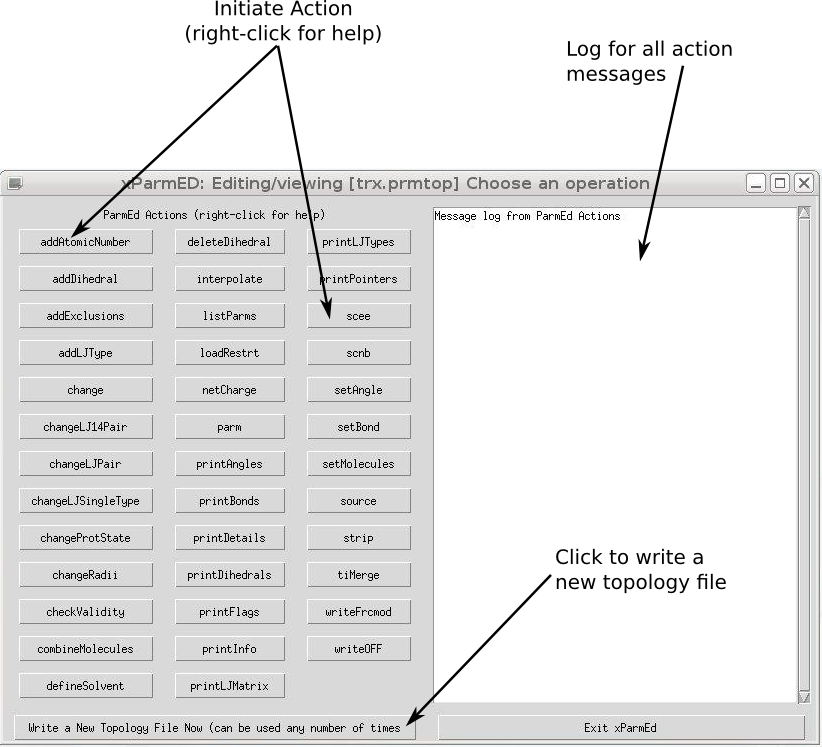
\includegraphics[width=6.5in, height=5.91in]{xparmed.png}
   \caption{Screenshot of the \emph{xparmed.py} GUI window, labeled with the
            available Actions and a message log.}
   \label{fig6:xparmed}
\end{figure}

The individual capabilities of ParmEd, called Actions, are all subclassed from a
common \emph{Action} base class. Each Action interprets its own list of
arguments and implements its own, unique functionality. To expand the utility of
the ParmEd code, users can incorporate individual ParmEd Actions into their own
Python script through an Application Programmer Interface (API) documented in
the AmberTools manual. This allows users to avoid the need to learn the
inner-workings of the prmtop file and re-implement existing code in the cases
where ParmEd does not handle all of the users' needs.

In the following sections, I will outline some of the Actions and functionality
I consider to be particularly helpful or particularly challenging to implement
through other programs.

\subsubsection{Lennard-Jones Parameter Modifications}

I will briefly describe here how the radius ($r_i$) and well depth
($\varepsilon_i$) assigned in the parameter databases for each atom type $i$ is
translated into a set of parameters used to compute the LJ potential in the
Amber force field. Specifically, between pairs $i$ and $j$, the well depth
$\varepsilon_{i,j}$ is the geometric average and the radius $r_{i,j}$ is the
arithmetic average
\begin{align}
   \varepsilon_{i,j} & = \sqrt{\varepsilon_i \varepsilon_j} \nonumber \\
   R_{min,i,j} & = R_{min,i} + R_{min,j}
   \label{eq6:CombiningRules}
\end{align}

These combined radii and depths are then combined into A-coefficients and
B-coefficients using the equations
\begin{align}
   ACOEF_{i,j} = \varepsilon_{i,j}r_{i,j}^{-12} \nonumber \\
   BCOEF_{i,j} = 2 \varepsilon_{i,j}r_{i,j}^{-6}
   \label{eq6:LJ}
\end{align}

Eqs. \ref{eq6:CombiningRules} and \ref{eq6:LJ} are evaluated in \emph{tleap},
and $\varepsilon_i$ and $r_i$ are provided as input in the parameter files.
Because there are more ACOEF and BCOEF parameters than there are input
parameters, the way \emph{tleap} handles LJ parameters restricts some
flexibility in the force field. The A and B coefficients can be thought of as a
matrix of pairwise combined terms---defined in Eq. \ref{eq6:LJ}---in which only
the diagonal terms are specified. The interactions between each pair of atom
types cannot be set independently like they can in the CHARMM program via the
\emph{NBFIX} keyword, for instance.

I will make a detour here to discuss how \emph{tleap} compresses the number of
LJ parameters written to the topology file. Since the LJ potential is composed
of pairwise terms, there must be a term for every pair of atoms in the
system---a number that becomes astronomically large for large numbers of
particles. To avoid printing out on the order of $N^2$ terms in both coefficient
matrices (where $N$ is the total number of atoms), \emph{tleap} assigns each
atom to a particular atom type index that it shares with every other atom in the
system that has the same set of starting LJ parameters $\varepsilon_i$ and
$r_i$. Therefore, each A- and B-coefficient printed in the topology file may be
used for numerous other atom pairs in the force and energy evaluations.

I implemented a number of Actions in ParmEd that allow users to query and adjust
LJ parameters in a way that is currently impossible with any other program. The
{\tt printLJTypes} Action in ParmEd takes an atom selection and prints out every
other atom that has been assigned to the same LJ atom type. The
\emph{changeLJPair} Action allows users to adjust individual, off-diagonal
elements of the A- and B-coefficient matrices for any pair of atoms. The
{\tt addLJType} command provides further flexibility by allowing the user to
treat a subset of atoms as a different LJ atom type so any off-diagonal changes
affect only the desired atoms.

\subsubsection{Changing Atomic Properties}

Another Action implemented in ParmEd---the {\tt change} Action---allows users to
change one of the following atomic properties: the partial charge, atomic mass,
implicit solvent radius, implicit solvent screening factor, atom name, atom type
name, atom type index, or the atomic number. Changing any of these properties
without using ParmEd requires the user to modify a number of files, including
standard residue libraries, force field databases, and the original starting
structure before running those files through \emph{tleap}. Even then, care must
be taken to ensure that the prmtop was changed the desired way.

This functionality allows rapid prototyping for tasks such as parameterizing new
charge or implicit solvent radius sets. Alternatives are currently tedious and
error-prone.

\subsubsection{Setting up for H-REMD Simulations}

The H-REMD implementation in Amber---described in Ch. \ref{ch5}---is capable of
performing alchemical REFEP calculations provided that the alchemical pathway
can be characterized by different topology files with the same atoms. When an
atom disappears---like in a pK\sub{a} calculation when a proton vanishes---a
dummy atom is required in the end state in which that atom is `missing.' The
{\tt interpolate} Action is provided to create a series of prmtops whose charge
and LJ parameters are linearly interpolated between two prmtops. Alternative
approaches are, again, time consuming and error-prone.

\subsubsection{Changing Parameters}

Perhaps one of the strongest features of ParmEd is its ability to change
individual bonded parameters---\ie bonds, angles, and torsions. The
{\tt setBond} and {\tt setAngle} commands can be used to either add or modify a
bond or angle parameter, respectively. The {\tt addDihedral} and
{\tt deleteDihedral} commands can be used to create, remove, and even change
individual torsion parameters. This control over the torsion parameters is
particularly useful when attempting to fit new torsion parameters to improve
force fields. \cite{Hornak_Proteins_2006_v65_p712,
Perez_BiophysJ_2007_v92_p3817, Lindorff-Larsen_Proteins_2010_v78_p1950}
